\documentclass[11pt]{article}
\usepackage[letterpaper,margin=1in]{geometry}
\usepackage{mathptmx,graphicx,booktabs,microtype}
\usepackage[authoryear,round]{natbib}
\usepackage[hidelinks]{hyperref}
\usepackage{caption}
\captionsetup{font=small,labelfont=bf}
\setlength{\parindent}{0pt}\setlength{\parskip}{6pt}
\newcommand{\FemaleN}{120}
\newcommand{\FemaleShare}{21.7}
\newcommand{\CohortOR}{1.65 (1.35--2.03)}
\newcommand{\JointYearOR}{1.99 (1.41--2.81)}
\newcommand{\RankAllOR}{0.66 (0.52--0.84)}
\newcommand{\RankCompleteOR}{0.67 (0.53--0.86)}
\newcommand{\RankJointOR}{1.33 (0.89--1.98)}
\newcommand{\TierOR}{0.87 (0.75--1.01)}
\newcommand{\TierAdjustedOR}{0.86 (0.74--1.003)}
\newcommand{\RecentOR}{1.38 (0.98--1.94)}
\newcommand{\PreTwentyOR}{1.63 (1.28--2.08)}
\newcommand{\OriginalCohortOR}{1.65 (1.35--2.03)}
\newcommand{\UnresolvedOR}{1.64 (1.34--2.02)}
\newcommand{\UGAdjustedOR}{1.75 (1.41--2.17)}
\newcommand{\FullCategoricalOR}{1.76 (0.79--3.89)}
\newcommand{\OverlapOR}{1.18 (0.48--2.86)}
\newcommand{\AssistantFemaleShare}{30.4}
\newcommand{\AssociateFemaleShare}{26.2}
\newcommand{\FullFemaleShare}{16.3}
\newcommand{\CohortOneFemaleShare}{10.8}
\newcommand{\CohortOneFemaleN}{16}
\newcommand{\CohortTwoFemaleShare}{25.0}
\newcommand{\CohortTwoFemaleN}{34}
\newcommand{\CohortThreeFemaleShare}{25.9}
\newcommand{\CohortThreeFemaleN}{44}
\newcommand{\CohortFourFemaleShare}{37.5}
\newcommand{\CohortFourFemaleN}{24}
\newcommand{\TierOneShare}{24.2}
\newcommand{\TierTwoShare}{33.3}
\newcommand{\TierThreeShare}{22.8}
\newcommand{\TierFourShare}{18.3}
\newcommand{\TierFiveShare}{18.0}

\title{\textbf{Gender Composition Across Doctoral Cohorts in US Transportation Engineering Faculty}}
\author{Andrew J.\ Bae\\[2pt]\small Department of Civil and Environmental Engineering, Carnegie Mellon University, Pittsburgh, PA, USA\\\small abae@alumni.cmu.edu\\\small ORCID: \href{https://orcid.org/0000-0002-7876-8998}{0000-0002-7876-8998}}
\date{}
\begin{document}\maketitle
\begin{abstract}
Among 553 transportation-focused faculty at 137 ranked US civil engineering institutions, \FemaleShare\% are classified female. The share is \CohortOneFemaleShare\% among doctorates completed by 1999 and \CohortFourFemaleShare\% among 2020--2025 doctorates. These are cohort differences within a January 2026 roster, not academic-entry rates. Rank differences become uncertain after cohort adjustment, with limited overlap between rank and cohort. Institutional-tier associations are also uncertain. Public-profile checks of 42 first-pass classifications identified one error, corrected here, and five unresolved cases. Differential classification error remains consequential; the roster cannot identify promotion, retention, or future parity.
\end{abstract}
\noindent\textbf{Keywords:} gender composition; transportation engineering; faculty; doctoral cohort; public records

\section*{QUESTIONS}
How does inferred gender composition vary across doctoral cohorts, faculty ranks, and institutional tiers in US transportation engineering? A common roster supports separate analyses of hiring prestige and geographic origins \citep{bae2026a,bae2026b}; this study adds a gender classification and examines its associations. The population is transportation-focused faculty in civil engineering departments, not the full multidisciplinary transportation workforce or a comparison with other engineering fields.

\section*{METHODS}
\textbf{Roster.} Public records describe a January 2026 snapshot. All 151 institutions in the 2026 US News civil engineering ranking frame were searched; 14 had no eligible transportation faculty, leaving 553 people at 137 institutions. Inclusion required a primary civil or civil-and-environmental engineering appointment and transportation or related mobility as a primary research/advising emphasis. Only tenure-track, tenured, and emeritus faculty were included; adjunct, research-only, teaching-only, and courtesy-only appointments were excluded. Emeritus faculty are coded as full professors. CVs took precedence over institutional pages, laboratory pages, and professional profiles. Supplement S1 supplies selection rules and the institutional frame.

\textbf{Classification.} A language model initially inferred likely binary gender using names and training context. The author checked 169 flagged faculty against public profiles; 384 classifications were initially accepted at high confidence. Original verification links were not retained. A new audit covered 42 first-pass records across cohorts and training backgrounds: public pronoun usage supported 36 labels, contradicted one, and was insufficient for five. The contradicted label was corrected; unresolved labels were retained provisionally and excluded in sensitivity analysis. Names and photographs alone were insufficient audit evidence. Benchmarks document errors in name-based inference \citep{santamaria2018}. This variable represents inferred binary classification, not self-identified gender, and does not capture nonbinary identities.

\textbf{Models.} Logistic regressions use individual doctoral year, scaled per decade, and rank coded assistant $=0$, associate $=1$, full $=2$. Thirty-five missing doctoral years are excluded only when year is required. Tier increases toward lower-ranked institutions: ranks 1--15, 16--30, 31--60, 61--100, and above 100. Ordinal rank and tier assume equal log-odds steps; categorical alternatives relax that assumption. Reported intervals are 95\% model-based confidence intervals conditional on roster membership and recorded attributes. S1 reports institution-clustered intervals, missing-year bounds, and directed classification-error scenarios. Cohort bins are descriptive; no future extrapolation is fitted.

\section*{FINDINGS}
\textbf{Cohorts.} After correction, \FemaleN{} of 553 faculty (\FemaleShare\%) are classified female. Known-year shares are \CohortOneFemaleShare\% (\CohortOneFemaleN/148) for 1999 or earlier, \CohortTwoFemaleShare\% (\CohortTwoFemaleN/136) for 2000--2009, \CohortThreeFemaleShare\% (\CohortThreeFemaleN/170) for 2010--2019, and \CohortFourFemaleShare\% (\CohortFourFemaleN/64) for 2020--2025 (Figure~\ref{fig:cohort}). The decade odds ratio is \CohortOR; retaining only 2000-onward doctorates gives \RecentOR. Thus recent growth and flattening remain difficult to distinguish. Earlier cohorts have had more time to retire, leave, or move outside the frame; recent doctorates have had less time to obtain appointments. Doctoral year is not appointment year.

\begin{figure}[ht]\centering
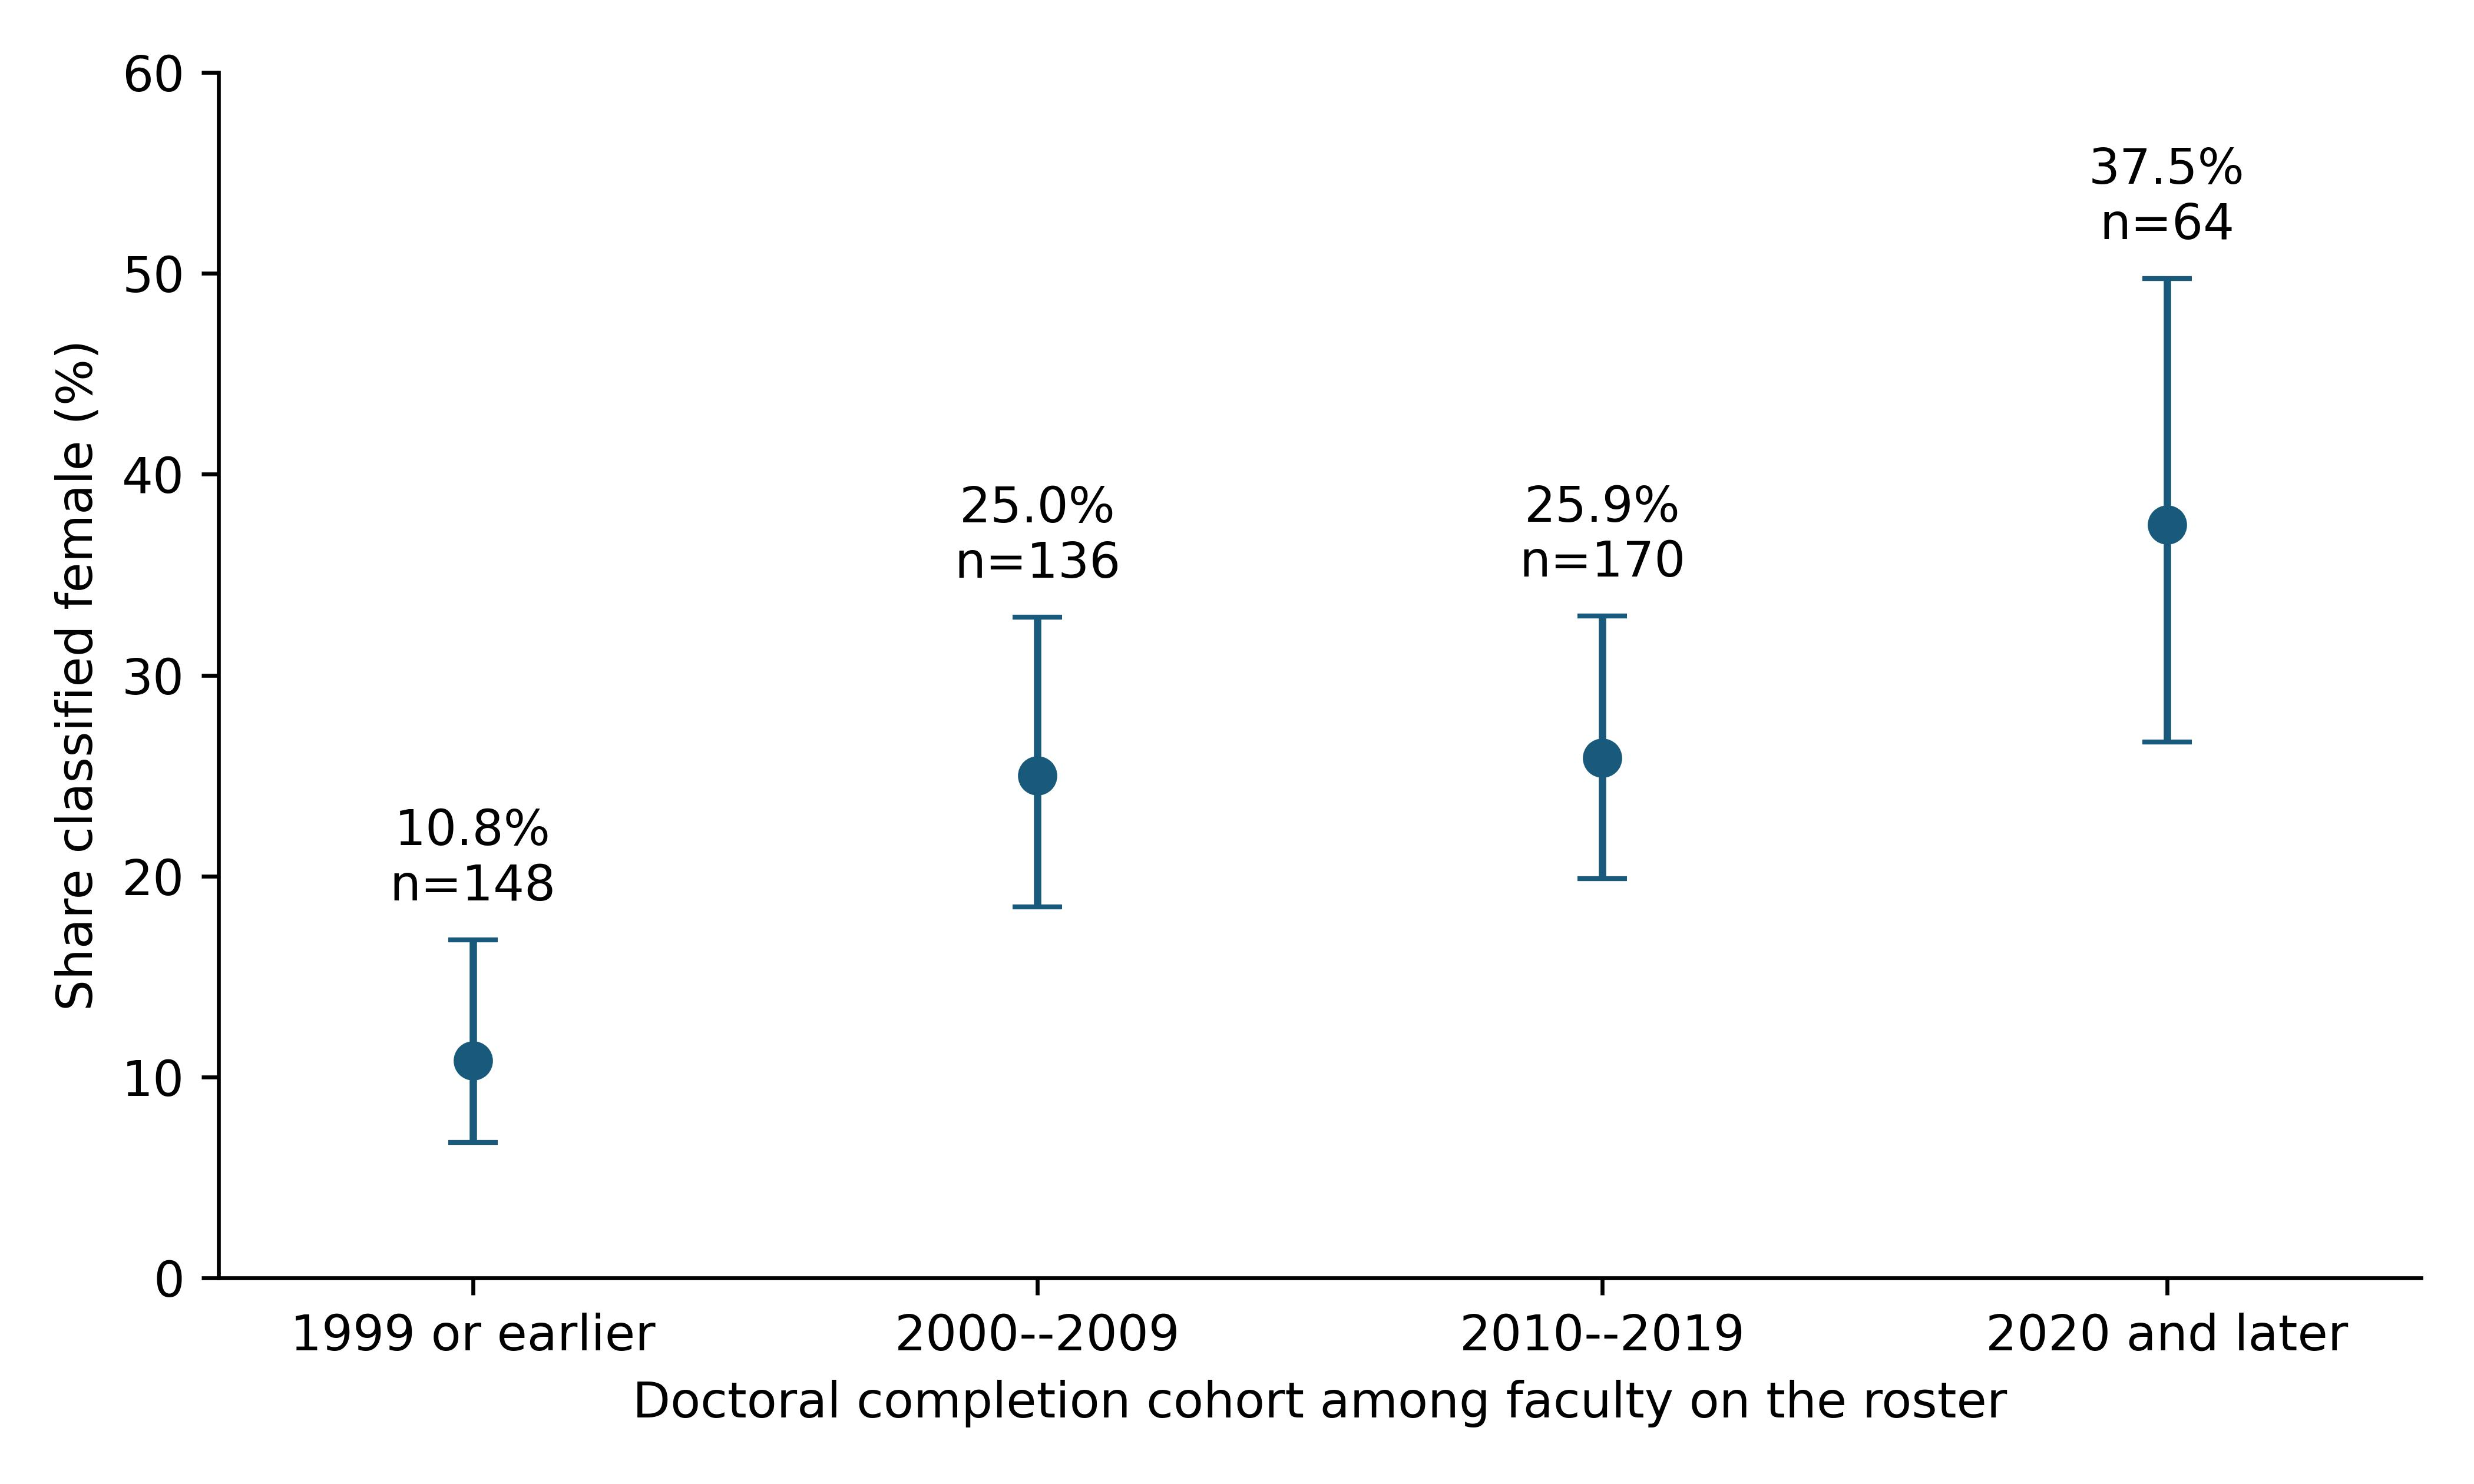
\includegraphics[width=.68\textwidth]{figures/Figure_1.jpeg}
\caption{Share classified female among rostered faculty with known doctoral year. Bars show 95\% Wilson intervals conditional on recorded labels. These are doctoral-cohort composition estimates, not academic-entry rates.}\label{fig:cohort}
\end{figure}

\textbf{Rank.} Female shares are \AssistantFemaleShare\% among assistants ($n=125$), \AssociateFemaleShare\% among associates ($n=122$), and \FullFemaleShare\% among full professors ($n=306$). On the same 518 observations, the rank odds ratio changes from \RankCompleteOR{} to \RankJointOR{} after cohort adjustment (Table~\ref{tab:models}). However, 142 of 148 pre-2000 doctorates are full professors, while all 64 post-2019 doctorates are assistants. Categorical rank adjustment gives full-versus-assistant odds ratio \FullCategoricalOR. These uncertain associations with limited overlap cannot identify promotion differences or their absence.

\begin{table}[ht]\centering\small
\caption{Odds ratios (95\% confidence intervals) for classification as female. Complete denotes known doctoral year.}\label{tab:models}
\resizebox{\textwidth}{!}{\begin{tabular}{lcccc}
\toprule
 & Cohort & Rank (all) & Rank (complete) & Joint \\
\midrule
Doctoral year (per decade) & 1.65 (1.35--2.03) & --- & --- & 1.99 (1.41--2.81) \\
Rank (per step) & --- & 0.66 (0.52--0.84) & 0.67 (0.53--0.86) & 1.33 (0.89--1.98) \\
$n$ & 518 & 553 & 518 & 518 \\
\bottomrule
\end{tabular}
}
\end{table}

\textbf{Institutional tier.} Female shares across tiers 1--5 are \TierOneShare\%, \TierTwoShare\%, \TierThreeShare\%, \TierFourShare\%, and \TierFiveShare\%. Tier 2 exceeds tier 1: the pattern is not monotonic. The overall tier odds ratio is \TierOR{}, or \TierAdjustedOR{} after cohort adjustment. These estimates describe affiliations, not hiring preferences.

\textbf{Robustness and limits.} Excluding the five unresolved audit records gives decade odds ratio \UnresolvedOR. Deliberately adverse changes to 19 remaining first-pass labels within cohorts reduce it to 1.18 (0.995--1.41); these are stress scenarios, not measured error rates. Webpage omissions, outdated profiles, and selective workforce survival remain unquantified. The data establish a descriptive cohort gradient within the roster, with classification uncertainty; they cannot separate entry, exit, and promotion processes.

\section*{ACKNOWLEDGMENTS}
Claude (Anthropic) assisted the initial classification, code, and drafting; OpenAI Codex assisted revision, source checks, and reanalysis. The author is responsible for the work.
\section*{DISCLOSURES}
No competing interests or financial support are declared. The analytical data, audit records, code, and instructions are in the separate Scholastica attachment labeled Replication data and code (\texttt{replication.zip}). Extract the archive and follow \texttt{README.txt}. The \href{https://github.com/werdnabae/transportation-faculty-doctoral-cohorts}{public replication repository} provides the data and code with individual profile links and excerpts removed. Attribute combinations and profile links can identify individuals.
\bibliographystyle{apalike}\bibliography{paper}
\end{document}
